\documentclass[main.tex]{subfiles}
\begin{document}
\section{Neutron Tagging with the analog setup}
\subsection{NE213 QDC spectrum}
1 hour of measurements $4.3\cdot 10^{6}$ events were recorded by the analog setup. Because the QDC baseline has been known to occasionally drift by tens of channels during acquisition it was necessary to inject pedestal into the QDC spectrum, in order to observe and compensate for any drift. This was done by allowing the acquisition start to trigger on YAP signals as well as NE213 signals. The number of YAP signals sent to the trigger was reduced by a factor of 256 with a prescaler. However, during this data run the pedestal remained stationary.

The uncalibrated QDC spectrum is shown in fig \ref{fig:qdc_a} top panel. The narrow peak located to the far left is the pedestal. It is produced when a YAP trigger gives a start signal causing the QDC module to integrate only the baseline. The bump immediately to the right of it is produced when the YAP trigger actually coincides with something. This may be the case when it was produced with a neutron or anotther gamma ray or when it scatters from the YAP and into NE213 detector.

The 2.23 and the 4.4 MeV Compton edges have been highlighted in green and red. Using the Knox method a linear fit has been made to these points and the pedestal as shown in fig \ref{fig:qdc_a} middle panel. From this fit the QDC channels have been converted to MeV electron equivalent. That is the amount of energy an electron would have had in order to produce a certain signal. The calibrated energy spectrum is shown in the bottom panel of fig \ref{fig:qdc_a}.
\begin{figure}[ht!]
    \centering
        \includegraphics{AnalogResults/Ecall.pdf}
        \caption{Top: The raw QDC spectrum. Middle: The callibration fit produced with the Knox method. Bottom: The energy calibrated QDC spectrum.}
    \label{fig:qdc_a}
\end{figure}

\subsection{Pulse Shape Discrimination}
Since neutrons and gammas interact differently in the NE213 detector their signal has different shape and duration. This makes it possible to discriminate between neutrons and gammas. The pulses were integrated over 500 ns and 60 ns and a constant 120 QDC channels was added to the shortgate QDC values, in order to linearize the pulse shape - Energy deposition spectrum. This corresponds to shifting the baseline of the signals during shortgate integration. No constant was added to the longgate QDC values.
\begin{figure}[ht]
    \centering
        \includegraphics{AnalogResults/psd.pdf}
        \caption{Heatmap of the fraction of total integrated charge as a function of energy. The dashed white line indicates the discrimination cut (tail/total = 0.259).}
        \label{fig:psd_a}
\end{figure}

\subsection{Time of Flight spectrum}
\begin{figure}[ht]
    \centering
        \includegraphics{AnalogResults/tof.pdf}
        \caption{The time calibrated time of flight spectrum. The x-axis denotes the time of flight from source to NE213 detector. The neutron and gamma peaks have been indicated with arrows and the upper right insert shows the energy distribution of events located in the neutron peak}
    \label{fig:A_TOF}
\end{figure}

\subsubsection{Pulse Shape and Time of Flight}
\begin{figure}[ht]
    \centering
        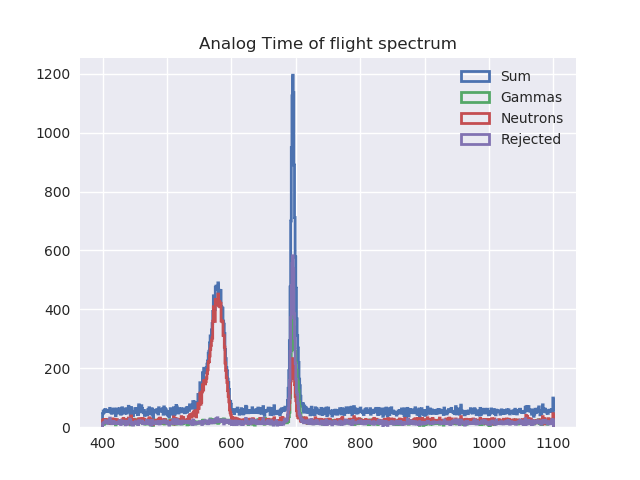
\includegraphics{AnalogResults/tof_psd.pdf}
        \caption{Time of flight plotted against fraction of charge located in the tail of signals. The dashed white line indicates the discrimination cut at tail/total = 0.259. A logarithmic z-axis is used to highlight the distribution of background events.}
    \label{fig:tof_ps_a} 
\end{figure}





\end{document}
